%! TEX program = lualatex

% This project should be between 5-6 pages.
% No cover page required.
% Font should be 12pt, with 3/4" margins on all sides.
% It should be properly written, divided into sections, 
% and must contain a proper introduction and bibliography.

\documentclass[12pt]{article}
%/========== Preamble ==========/%
% Set Margins to 3/4"
\usepackage[margin=0.75in]{geometry}

%---------- Math Packages ----------%
\usepackage{amsmath}
\usepackage{amssymb}
\usepackage{mathtools}
\usepackage{amsthm}

%---------- Minipage ----------%
\usepackage{graphicx}
\usepackage{caption}

% Define theorem styles
\newtheorem{thm}{Theorem}
\newtheorem{prop}{Proposition}
\newtheorem*{cor}{Corollary}

\theoremstyle{definition}
\newtheorem{defn}{Definition}
\newtheorem{example}{Example}
\newtheorem*{notation}{Notation}

%---------- Bibliography Style ----------%
\usepackage[style=ieee,backend=biber]{biblatex}
\addbibresource{bib.bib}

%/========== Main Document ==========/%
\begin{document}
    
\section{Introduction}
One common approach to controlling robotic manipulators 
(known colloquially as ``robot arms") is to pick a pose of the end effector and
reverse-engineer the joint angles required to reach this pose. This is known as
the \textbf{inverse kinematics} problem. For an arm with \(n\) rotating 
(also known as revolute) joints, one can model the desired end effector position
and orientation by \(x \in \mathbb{R}^3 \times SO(3)\) and the angles of the
joints by \(\theta \in \mathbb{T}^n\) \cite{robots-fiber-bundles}. 
The inverse kinematics problem requires solving the
equation \(f(\theta) = x\) for \(\theta\), where \(f\) is an 
appropriately-defined function \cite{program-kin-red-manips}.

Unfortunately, there always exist joint angles where the relationship 
\(x = f(\theta)\) breaks down. These points are called 
\textbf{singular configurations}. If the dimension of the workspace is 
\(k > 0\), the singular configurations are characterized by the set
\[
    S = \left\{ \theta_0 \in \mathbb{T}^n \mid 
    \text{rank}\left\{
        \frac{\partial f}{\partial\theta}(\theta_0) 
    \right\} < k \right\}
\]

\begin{example}
%TODO: the 2D planar manipulator image.
    The 2D planar manipulator with two revolute joints of fixed lengths \(r_1 > 0\)
    and \(r_2 > 0\) (Figure \ref{fig:2-link-arm}), whose end-effector's orientation is the same
    as the second joint's, has position \((x,y) \in \mathbb{R}^2\) and joint angles 
    \(\theta = (\theta_1,\theta_2) \in \mathbb{T}^2\). 
    The relation connecting these two is given by (\ref{eqn:2d-planar-manip}).
    \begin{equation}\label{eqn:2d-planar-manip}
        \begin{bmatrix}x \\ y \end{bmatrix}
        = \begin{bmatrix} 
            r_1\cos(\theta_1) + r_2\cos(\theta_1 + \theta_2) \\
            r_1\sin(\theta_1) + r_2\sin(\theta_1 + \theta_2)
        \end{bmatrix} =: f(\theta)
    \end{equation}
    The Jacobian has determinant
    \[
        \left| \frac{\partial f}{\partial \theta} \right| = r_1r_2\sin(\theta_2)
    \]
    which means the singular configurations are 
    \(S = \left\{ (\theta_1,\theta_2) \in \mathbb{T}^2 \mid \theta_2 = \pm\pi\right\}\); 
    that is, the singular configurations of this robot arm are exactly when the
    second joint is colinear with the first joint.
\end{example}

Singularities cause various issues when controlling robot arms, as the
controllers will attempt to apply infinite torque to move the arm a 
small amount. For this reason, it is preferable
to avoid singular configurations when possible. In particular, when generating a
trajectory for the end-effector, a good control mechanism should avoid choosing
joint positions which land ``close to" the singular configurations.

Previous researchers have tried to solve this problem using extra limbs
\cite{program-kin-red-manips} and velocity constraints
\cite{articulated-robot-redundancy}, among other approaches involving kinematic
models of the robots. The authors of
``Topology and the Robot Arm" offer a different approach: they ask whether
avoiding kinematic singularities is possible at all, and prove when it can be
done using the topology of the robot's configuration space
\cite{topology-robot-arm}.

This report will cover the relevant background required to understand 
``Topology and the Robot Arm",
and will summarize the results of the paper.

\begin{figure}
    \centering
    \begin{minipage}{.45\textwidth}
        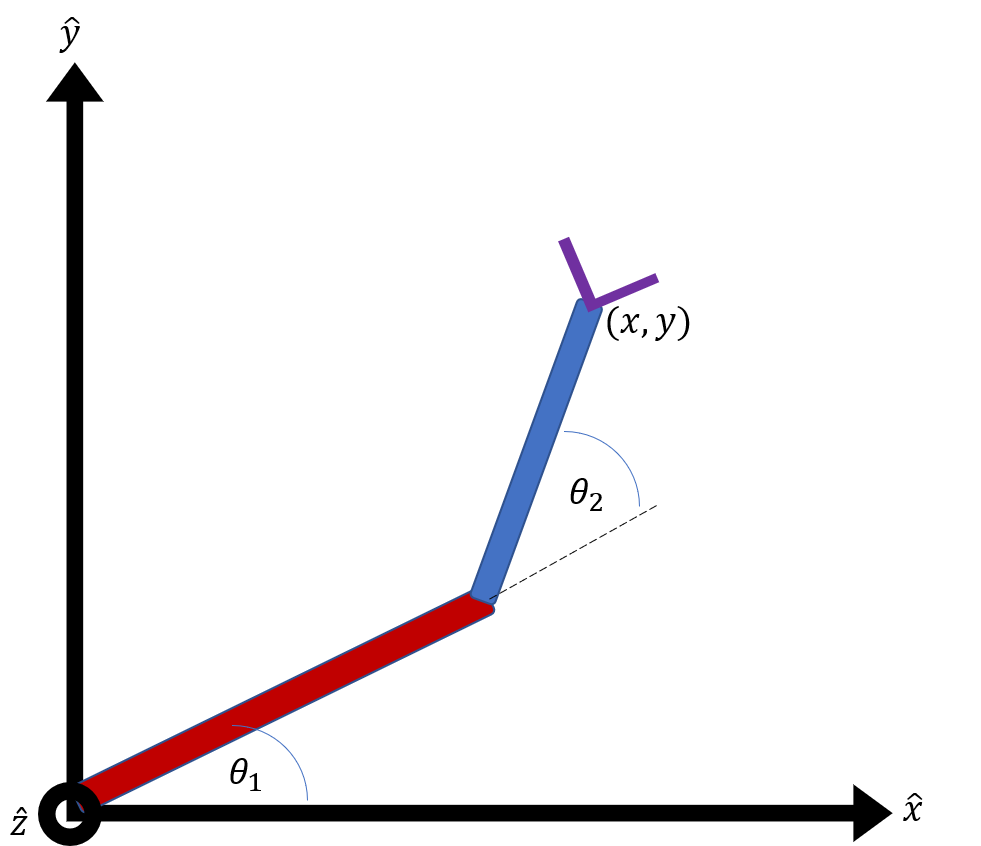
\includegraphics[width=0.8\linewidth]{images/robot-arm.png}
        \captionof{figure}{A 2D planar robot arm with fixed lengths and a
        non-rotating end-effector.}\label{fig:2-link-arm}
    \end{minipage}
    \hfill
    \begin{minipage}{.45\textwidth}
        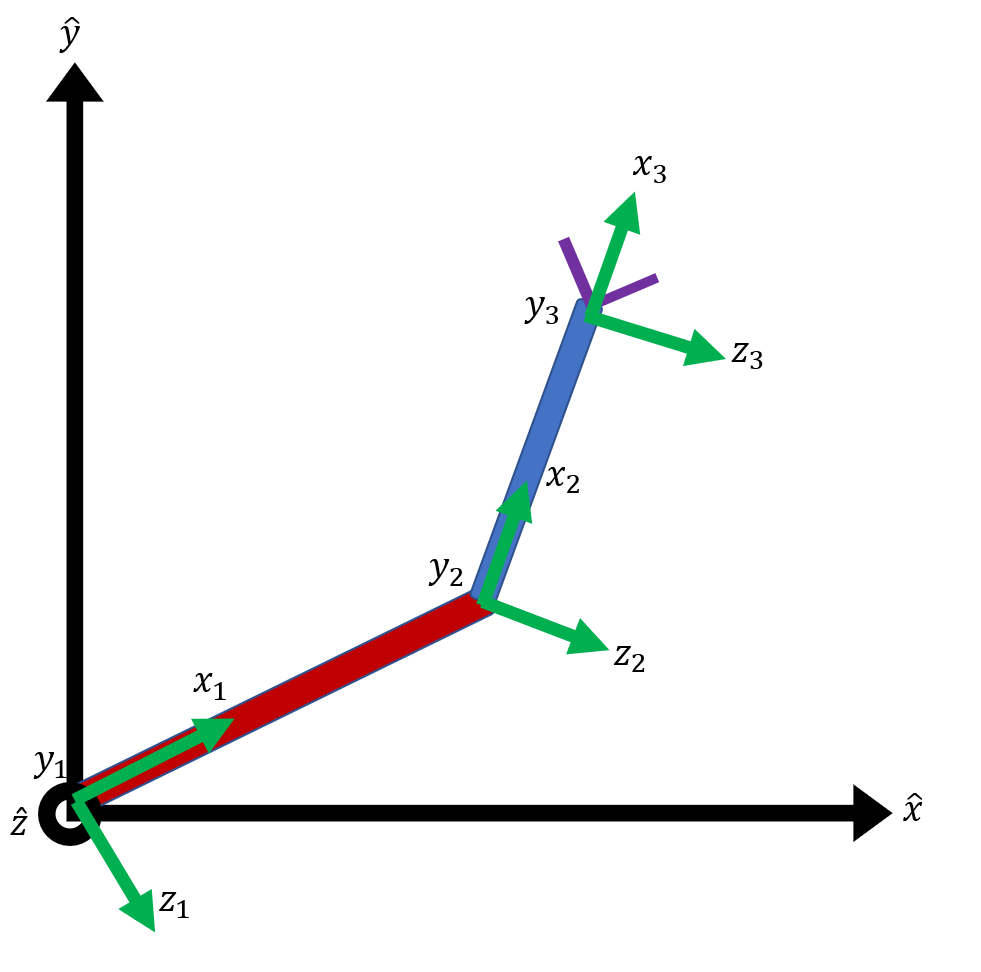
\includegraphics[width=0.8\linewidth]{images/robot-arm-frames.png}
        \captionof{figure}{The planar robot arm with coordinate frames attached to each pivot
    \(y_i\).}\label{fig:planar-singular-frames}
    \end{minipage}
\end{figure}

\section{Relevant Background}
This section covers definitions, notation, and results that are required to
fully comprehend \cite{topology-robot-arm}. It is assumed that anyone reading
this report will have completed the material of MAT327 as taught in the summer
of 2020.

\begin{defn}[Fiber bundles \cite{topology-fiber-bundles}]
    Let \(E\), \(X\), and \(F \subset E\) be topological spaces, 
    with \(X\) connected.
    Let \(f : E \rightarrow X\) be a continous surjective function. 
    We say \(f\) is a \textbf{locally trivial fibration} or a 
    \textbf{fiber bundle with fiber \(F\)} and write 
    \(F \rightarrow E \xrightarrow[]{f} X\) when
    \begin{enumerate}
        \item \(f^{-1}(\{x_0\}) = F \, \forall x_0 \in X\)
        \item \((\forall x \in X)\) there is an open neighbourhood of \(x\)
            \(U_x \subset X\) and a homeomorphism
            \(\psi_x : f^{-1}(U_x) \rightarrow U_x \times F\) so that
            \(f\vert_{f^{-1}(U_x)} = \pi_1 \circ \psi_x\) (where \(\pi_1\)
            is the projection map of \(U_x \times F\) onto \(U_x\))
    \end{enumerate}
    Note that it is common to say that \(E\) itself is the fiber bundle over
    \(X\) if \(E = X \times F\), since the natural projection 
    \(\pi : X \times F \rightarrow X\) is a fiber bundle.
\end{defn}

\begin{defn}[Vector bundles \cite{topology-fiber-bundles}]
    Let \(V \rightarrow E \xrightarrow[]{f} E\) be a fiber bundle and \(V\) an
    \(n\)-dimensional vector space. We say \(f\) is a
    \textbf{vector bundle} if \(\psi_x\) satisfies
    \(\psi_x \vert_{x_1} : f^{-1}(x_1) \rightarrow {x_1}\times V\) is a linear
    isomorphism for any \(x_1 \in U_x\).
\end{defn}

\begin{defn}[Cross-sections \cite{topology-fiber-bundles}]
    Let \(F \rightarrow E \xrightarrow[]{f} X\) be a fiber bundle.
    A \textbf{cross-section} is a continuous map \(\sigma : X \rightarrow E\)
    such that \(f \circ \sigma = \text{id}_X\).
\end{defn}

\begin{defn}[Bundle maps \cite{topology-fiber-bundles}]
    Let \(F_1 \rightarrow E_1 \xrightarrow[]{f_1} X_1\) and 
    \(F_2 \rightarrow E_2 \xrightarrow[]{f_2} X_2\) be fiber bundles. A
    continuous function \(\phi : E_1 \rightarrow E_2\) is a \textbf{bundle map}
    if there is a continuous function \(g : X_1 \rightarrow X_2\) so that
    \(g \circ f_1 = f_2 \circ \phi\).
\end{defn}

\begin{defn}[Pullback \cite{topology-fiber-bundles}]
    Let \(F \rightarrow E \xrightarrow[]{f} X\) be a fiber bundle. Let \(Y\) be
    a topological space and \(g : Y \rightarrow X\) a continuous function. The
    \textbf{pullback bundle over \(Y\)} is 
    \(g^\star(E) := \left\{ (y,e)\in Y \times E \mid g(y) = f(e)\right\}\). The
    natural projection \(\pi_Y : g^\star(E) \rightarrow Y\) with 
    \((y,e) \mapsto y\) is a fiber bundle with fiber \(F\).
\end{defn}

\begin{defn}[Manifolds \cite{intro-top-manifolds}]
    A topological space \(M\) is a manifold of dimension \(n\) if for any
    \(p \in M\) there exists an open neighbourhood \(U \subset M\) of \(p\)
    which is homeomorphic to an open subset of \(\mathbb{R}^n\).
\end{defn}

\begin{defn}[Tangent Bundles \cite{geometric-control}]
    Let \(M\) be a manifold and \(m \in M\). The set \(T_mM\) consisting of
    tangents of curves at \(m\) is called the \textbf{tangent space} of \(M\) at
    \(m\). The set \(TM := \left\{(m,v) | m \in M,\, v \in T_mM\right\}\) is
    called the \textbf{tangent bundle} of \(M\).
\end{defn}

\begin{example}\label{ex:tangent-bundle}
    A mechanical system can be modelled by a configuration manifold
    \(\mathcal{Q} = \mathbb{R}^n \times (\mathbb{S}^1)^m\). At each
    \(q \in \mathcal{Q}\), the velocity of the system lies in
    \(T_q\mathcal{Q}\), which is an \(n+m\)-dimensional vector
    space. 
    The tangent bundle
    \(T\mathcal{Q} := \left\{(q,v) \mid q \in \mathcal{Q}, v \in
    T_q\mathcal{Q}\right\}\)  has the natural
    projection \(\pi : T\mathcal{Q} \rightarrow \mathcal{Q}\) given by 
    \(\pi(q,v) = q\). This is a vector bundle, because the fibers 
    \(\pi^{-1}(q) = T_q\mathcal{Q}\) are isomorphic to 
    \({q} \times \mathbb{R}^{n+m}\).
\end{example}

\begin{defn}[Submersions \cite{robots-fiber-bundles}]
    Let \(M\) and \(N\) be manifolds. A map \(h : M \rightarrow N\) is a
    \textbf{submersion} if it contains no singular points (that is, its Jacobian
    is always full rank).
\end{defn}

\begin{defn}[Groups \cite{intro-top-manifolds}]
    A \textbf{group} is a set \(G\) and an operation 
    \(\cdot : G\times G \rightarrow G\) with \((g,h) \mapsto gh\), along with
    the following axioms:
    \begin{enumerate}
        \item For all \(g,h,k \in G\), \((gh)k = g(hk)\).
        \item There exists an identity \(e \in G\) so that for all \(g \in G\)
            we have \(eg = ge = g\).
        \item For all \(g \in G\) there is an inverse \(h \in G\) so that
        \(gh = e\)
    \end{enumerate}
    If additionally the group satisfies \(gh = hg\) for all \(g,h \in G\), the
    group is called \textbf{abelian}.
\end{defn}

\begin{defn}[Group Homomorphism \cite{intro-top-manifolds}]
    Let \(G\) and \(H\) be groups. A function \(f : G \rightarrow H\) is a
    \textbf{homomorphism} if \(f(g_1g_2) = f(g_1)f(g_2)\) for all 
    \(g_1,g_2 \in G\).
\end{defn}

\begin{defn}[Group Torsion \cite{intro-top-manifolds}]
    An abelian group \(G\) is a \textbf{torsion group} if for each \(g \in G\),
    there exists \(n \in \mathbb{N}\) so that \(g^n = e\). If this is not the
    case, \(G\) is said to be \textbf{torsion-free}.
\end{defn}

\begin{defn}[Quotient Group \cite{intro-top-manifolds}]
    Let \(g \in G\) and \(H \subset G\). Define \(g \equiv g' (\text{mod } H)\)
    if and only if \(g^{-1}g' \in H\). The set of equivalence classes mod \(H\)
    is denoted \(G/H\).
\end{defn}

\begin{defn}[Group Commutator \cite{intro-top-manifolds}]
    Let \(G\) be a group. The \textbf{commutator subgroup}, denoted \([G,G]\),
    is the subgroup of \(G\) generated by the elements of the form
    \(a b a^{-1} b^{-1}\) for \(a,b \in G\)
\end{defn}

\begin{defn}[Exact Sequence \cite{intro-top-manifolds}]
    A sequence of abelian groups \(\{G_1, G_2, \ldots\}\) and
    homomorphisms \(\alpha_p : G_p \rightarrow G_{p-1}\)
    \[
        \cdots \rightarrow G_{p+1} \xrightarrow{\alpha_{p+1}} G_p
    \xrightarrow{\alpha_p} G_{p-1} \rightarrow \cdots
    \]
    is \textbf{exact} if \(\text{Image}(\alpha_{p+1}) = \text{Ker}(\alpha_p)\)
    for all \(p\).
\end{defn}

\begin{prop}[Homotopy Groups \cite{topology-fiber-bundles}]
    The homotopy group \(\pi_n(X,x_0)\) of \(n\)-loops at \(x_0\) is the
    set of equivalence classes of maps from \(\mathbb{S}^n\) to \(X\) with the
    homotopy group operation (as defined in \cite{intro-top-manifolds}).
\end{prop}

\begin{notation}
    The notation \(g : (Y,C,y_0) \rightarrow (X,A,x_0)\) (used in 
    \cite{topology-fiber-bundles}) means that \(g : Y \rightarrow X\), 
    \(g(C) = A\), \(y_0 \in C\) and \(g(y_0) = x_0 \in A\).
\end{notation}

\begin{notation}
    Let \(g : (D^n, \mathbb{S}^{n-1},t_0) \rightarrow (X,A,x_0)\). 
    The restriction of \(g\) to the sphere \(\mathbb{S}^{n-1}\) is denoted by 
    \(\partial g : (\mathbb{S}^{n-1},t_0) \rightarrow (A,t_0)\)
    \cite{topology-fiber-bundles}.
\end{notation}

\begin{prop}[Boundary Homomorphism \cite{topology-fiber-bundles}]
    The function \(\partial g : (\mathbb{S}^{n-1},t_0) \rightarrow (A,t_0)\)
    defines a homomorphism 
    \(\partial_* : \pi_n(X,A,x_0) \rightarrow \pi_{n-1}(A,x_0)\).
\end{prop}

\begin{defn}[Relative Homotopy Group \cite{topology-fiber-bundles}]
    The relative homotopy group \(\pi_n(X,A,x_0)\) is the set of equivalence classes
    of the maps \(g : (D^n,\mathbb{S}^{n-1},t_0) \rightarrow (X, A, x_0)\)
    where \(D^n\) is the \(n\)-disk.
\end{defn}

\begin{defn}[Homotopy-Exact sequence \cite{topology-fiber-bundles}]
    Let \(F \rightarrow E \xrightarrow{f} X\) be a locally trivial fibration and suppose
    \(\iota : F \rightarrow E\) is the inclusion map of the fiber.
    The \textbf{homotopy-exact sequence} of this fibration is the exact sequence
    \[
        \cdots \rightarrow \pi_n(F) \xrightarrow{\iota_*} \pi_n(E) 
        \xrightarrow{f_*} \pi_n(X) \xrightarrow{\partial_*} \pi_{n-1}(F)
        \rightarrow \cdots
    \]
\end{defn}

\begin{defn}[Homology \cite{topology-fiber-bundles}]
    The \textbf{first homology group} \(H_1(X)\) of a space \(X\) the set
    characterized by the  abelianization of the fundamental group \(\pi_1(X)\):
    \[
        H_1(X) \equiv \pi_1(X)/[\pi_1,\pi_1]]
    \]
\end{defn}

\begin{notation}
    The notation
    \(f : X \xrightarrow{\alpha} Y \xrightarrow{\beta} Z\)
    in \cite{topology-robot-arm} means that \(f = \beta \circ \alpha\) where
    \(\alpha : X \rightarrow Y\) and \(\beta : Y \rightarrow Z\).
\end{notation}

\begin{thm}[Ehresmann's Theorem \cite{ehresmann}]
    Let \(M\) and \(N\) be smooth manifolds, with \(M\) a compact. 
    Let \(f : M \rightarrow N\) be a surjectie submersion. Then \(f\) is a
    locally trivial fibration.
\end{thm}

\section{Topology and the Robot Arm}
This section covers a summary of \cite{topology-robot-arm}. I will not cover
all proofs of the results from this paper. When possible I
will try to motivate why the results are true by using concrete examples.

\subsection{The Global Inverse Kinematics Problem}
At the start of the paper, he authors note that a robot arm can be represented
by a series of links. Let \(l_1\) be the first link in the robot arm, which is
attached to the base and can rotate about the fixed line \(y_1\) in 3D space.
Then, attach a new link \(l_2\) to the end of \(l_1\) and pick a line \(y_2\)
around which \(l_2\) will rotate. Building this up inductively, one creates a
robot arm so that \(y_{i+1}\) rotates about \(y_i\). The orientation of the
end-effector is described by a coordinate frame attached to the end of the link
\(l_n\), whose \(x\)-axis is colinear with \(y_n\).

\begin{example}
    The 2D planar robot from Figure \ref{fig:2-link-arm} has 
    \(y_1 = y_2 = \hat{z}\).
\end{example}

Since the end-effector's pose can be represented by a point in
\(\mathbb{R}^3\times SO(3)\), the authors define the ``rotation map" 
\(R : \mathbb{T}^n \rightarrow SO(3)\) as follows: 
given \(\theta = (\theta_1,\ldots,\theta_n) \in \mathbb{T}^n\),
the map \(R(\theta)\) rotates \(l_i\) about \(y_i\) by the angle \(\theta_i\)
and returns the orientation of the end-effector (ignoring its position in
3D-space). Here it is assumed that rods cannot collide with each other, which
is a reasonable assumption as many robot arms are designed so that each limb can
rotate completely without breaking the system.

Now we arrive at the first theorem of the paper, which characterizes the singular
configurations of the map \(R\) in terms of the physical representation of the
axes.

\begin{thm}\label{thm:singular-plane}
    A point \(\theta \in \mathbb{T}^n\) is a singular configuration for \(R\) if
    and only if the axes \(\{y_1,\ldots,y_n\}\) are parallel to a plane.
\end{thm}
\begin{cor}
    The set of singularities \(S \subset \mathbb{T}^n\) is 2-dimensional.
\end{cor}

The phrasing of Theorem \ref{thm:singular-plane} is somewhat confusing when we
look at the 2D planar robot: any configuration has the axes in some plane since \(y_1\) and
\(y_2\) are connected by the link \(l_1\). 
In this case, we need to add an additional ``axis" (which cannot rotate) labelled
\(y_3\) at the end of the arm. If these three lines \(y_1\), \(y_2\), and \(y_3\)
are all in the same plane, the robot must have \(\theta_2 = \pm \pi\) and it
must be in a singular configuration. This is shown in Figure
\ref{fig:planar-singular-frames}, where the lines \(y_i\) are perpendicular to the
green coordinate frames.
To see that the set of singular configurations is 2D, observe that rotating by
\(y_1\) keeps the axes in a plane, as would any hypothetical rotation of the
end-effector about \(y_3\).

Next, the authors make the claim that we can create a homotopy of robot arms.
Letting \(\phi_i\) be the angle between \(y_{i+1}\) and \(y_i\), they construct
the homotopy by shrinking each \(\phi_i\) until we get an \(n\)-link planar
robot arm. In this case, the coordinate frame on the end-effector has an 
\(x\)-axis which is fixed to be colinear with \(y_1\) (as is the case with our
2-link planar arm). This gives us the homotopy \(R \sim R_1\), where \(R_1\)
rotates the end-effector rotates about this fixed \(x\)-axis when any link
is rotated. The amount of rotation is 
\(\theta' = \theta_1 + \cdots + \theta_n \in \mathbb{S}^1\). This addition of
angles is the group operation on \(\mathbb{S}^1\), so we represent this by a map
\(\mu : \mathbb{T}^n \rightarrow \mathbb{S}^1\). 

Letting \(\alpha : \mathbb{S}^1 \rightarrow SO(3)\) be the rotation map around
the \(x\)-axis, we can now state the next result.
\begin{thm}
    A robot arm map \(R : \mathbb{T}^n \rightarrow SO(3)\) is homotopic to 
    the composition 
    \(\mathbb{T}^n \xrightarrow{\mu} \mathbb{S}^1 \xrightarrow{\alpha} SO(3)\)
    where \(\mu\) is the group operation on \(\mathbb{S}^1\) and \(\alpha\) is a
    group generator for \(\pi_1\left(SO(3)\right)\).
\end{thm}

That \(R\) is homotopic to the composition and \(\mu\) is the group operation on
\(\mathbb{S}^1\) comes from the previous discussion. The proof that \(\alpha\)
is the group generator for the fundamental group of \(SO(3)\), however, is more
obtuse, and I do not understand the proof enough to explain it in this report. 

Let now \(w : SO(3) \rightarrow \mathbb{S}^2\) be the map which takes a rotated
coordinate frame and returns its \(x\)-axis (in the sense that the tip of the
\(x\)-axis vector lies along a sphere).
Since \(R\) is homotopic to \(R_1\), 
\(w \circ R : \mathbb{T}^n \rightarrow \mathbb{S}^2\) is homotopic to 
\(w \circ R_1\), which is constant because the \(x\)-axis of \(R_1\) is
constant. The authors claim \(w\) creates a fiber bundle 
\(\mathbb{S}^1 \rightarrow SO(3) \xrightarrow{w} \mathbb{S}^2\), which is a fact
we will take for granted. This leads us to one of the most important results in
this paper.

\begin{cor}
    There is no continuous cross-section to \(R\) or to \(w \circ R\).
\end{cor}
\begin{proof}
    In this context, the cross-section is a continuous map 
    \(s : SO(3) \rightarrow \mathbb{T}^n\) so that \(R \circ s = \text{id}\). 
    Looking at the fundamental groups, existence of a cross-section would imply
    that \(R_* \circ s_* = \text{id}_{\pi_1(SO(3)}\). This is impossible, since
    \(\pi_1(\mathbb{T}^n)\) is torsion-free, while
    \(\pi_1(SO(3))\) is the cyclyc group of order 2 (which has torsion). 
    If \(w \circ R\) had a cross-section \(s'\), then \(\text{id}_\mathbb{S}^2\)
    would be homotopic to a constant (which it is not).
\end{proof}

Finding a cross-section to \(R\) is equivalent to finding a continuous map which
gives joint angle \(\theta \in \mathbb{T}^n\) for any end-effector orientation.
In other words, this corollary tells us there is no global, continuous solution
to the inverse kinematics problem.

\subsection{Avoiding Singularities}
The rest of the paper focuses on solving the inverse kinematics problem while
avoiding singularities. 
The authors suggest finding some set \(D\) and a map \(\hat{f} : D \rightarrow
\mathbb{T}^n - S\) so that \(R \circ \hat{f}\) has no singularities.

\begin{prop}
    If \(D\) is a closed manifold, \(R \circ \hat{f}\) will have singularities.
\end{prop}
\begin{proof}
    Suppose \(R \circ \hat{f}\) has no singularities. Then neither will 
    \(w \circ R \circ \hat{f} : D \rightarrow \mathbb{S}^2\), since \(w\) is a
    projection map of a fiber bundle. By definition, 
    this means \(w \circ R \circ \hat{f}\) is a submersion.
    By Ehresmann's theorem, since \(D\) and \(\mathbb{S}^2\) are closed
    manifolds, \(w \circ R \circ \hat{f}\) is a locally trivial fibration with
    some fiber \(F\).
    Let \(\Omega\mathbb{S}^2\) be the set of all loops based in X (the ``loop
    space").
    The authors claim \(F\) must be a finite-dimensional manifold homotopic to
    \(D \times \Omega\mathbb{S}^2\) because \(w \circ R \circ \hat{f}\) is
    homotopic to the constant map \(w \circ R_1 \circ \hat{f}\). I was unable to
    find a source on this claim, so we will take it as fact.
    Since homology groups are preserved under homotopy \cite{intro-top-manifolds}, and
    the homology group of finite-dimensional manifolds is finite dimensional, the
    homology of \(D \times \Omega\mathbb{S}^2\) must also be finite
    dimensional. The authors claim this is not true (I could not find
    a good source proving this claim), giving a contradiction.
\end{proof}

Finally, let \(E = TSO(3)\) be the (trivial) tangent
bundle of \(SO(3)\) with projection map \(p_E\). Let \(D = T(\mathbb{T}^n - S)\) be
the tangent bundle of \(\mathbb{T}^n - S\) with projection map \(p_D\).
Let \(R^*E\) be the pullback bundle of \(R|_{\mathbb{T}^n - S}\) onto
\(\mathbb{T}^n - S\) with projection \(p_R\). 
Then \(D\) is the set of position-velocity pairs
\((\theta, v_\theta)\) in joint space, and \(R*E\) is the set of pairs
\((\theta, v_{R(\theta)})\) where \(v_{R(\theta)} \in T_{R(\theta)}SO(3)\) 
is a velocity at the current orientation. 
Given a starting orientation \(R(\theta_0)\), the existence of a
cross-section \(s : R^*E \rightarrow D\) would find the velocity in joint space
required to produce a desired velocity and position in the orientation (all while
avoiding singular configurations). By the results of
\cite{robots-fiber-bundles}, this cross-section exists, so the inverse
kinematics problem can be solved.

\section{Conclusion}
This report compiles the relevant bacground information to understand the paper
``Topology and the Robot Arm"
\cite{topology-robot-arm} and summarizes the results of that paper.
We find it is only possible to solve the inverse kinematics problem 
by omitting singular configurations.

%---------- Bibliography ----------%
%\newpage
% This adds a line for the Bibliography in the Table of Contents.
\addcontentsline{toc}{chapter}{Bibliography}
\printbibliography
\end{document}
%/========== /Main Document ==========/%

% vim: set tw=80 ts=4 sw=4 sts=0 et ffs=unix :
